% XeLaTeX can use any Mac OS X font. See the setromanfont command below.
% Input to XeLaTeX is full Unicode, so Unicode characters can be typed directly into the source.

% The next lines tell TeXShop to typeset with xelatex, and to open and save the source with Unicode encoding.

%!TEX TS-program = xelatex
%!TEX encoding = UTF-8 Unicode

\documentclass[11pt,twoside,openany]{book}
\usepackage{multirow}
\usepackage{pdfpages}

\usepackage{xspace}

\usepackage{array}
\usepackage{lipsum}

\usepackage{algorithm}
\usepackage{algpseudocode}

\usepackage{geometry}                % See geometry.pdf to learn the layout options. There are lots.
%\usepackage[margin=1cm]{geometry}


% \addtolength{\textwidth}{1.75in}
%
% \addtolength{\topmargin}{-.875in}
% \addtolength{\textheight}{1.75in}

\geometry{a4paper,left=20mm,top=20mm,bottom=50mm,total={162mm,230mm}}                   % ... or a4paper or a5paper or ...
%\geometry{landscape}                % Activate for for rotated page geometry
%\usepackage[parfill]{parskip}    % Activate to begin paragraphs with an empty line rather than an indent
\usepackage{amssymb}
%\usepackage{todonotes}
\setlength{\marginparwidth}{2cm}
\usepackage[backgroundcolor=white,bordercolor=blue,linecolor=blue,textwidth=1cm]{todonotes}
\usepackage{booktabs}
\usepackage{longtable}
\usepackage{url}

\usepackage[depth=4]{bookmark}


\usepackage{algorithm}
\usepackage{algpseudocode}

\usepackage{imakeidx}
\usepackage[utf8]{inputenc}
\usepackage[T1]{fontenc}
\makeindex[intoc]

\usepackage[font=normalsize]{caption}

\renewcommand{\theparagraph}{\S\arabic{paragraph}}
\setcounter{secnumdepth}{4}


\usepackage{xcolor}
\usepackage{listings}

\makeatletter
\global\let\tikz@ensure@dollar@catcode=\relax
\makeatother

\definecolor{mGreen}{rgb}{0,0.6,0}
\definecolor{mGray}{rgb}{0.5,0.5,0.5}
\definecolor{mPurple}{rgb}{0.58,0,0.82}
\definecolor{backgroundColour}{rgb}{0.95,0.95,0.92}
\definecolor{gray}{rgb}{0.4,0.4,0.4}
\definecolor{darkblue}{rgb}{0.0,0.0,0.6}
\definecolor{cyan}{rgb}{0.0,0.6,0.6}

\lstdefinestyle{CStyle}{
    backgroundcolor=\color{backgroundColour},
    commentstyle=\color{mGreen},
    keywordstyle=\color{magenta},
    numberstyle=\tiny\color{mGray},
    stringstyle=\color{mPurple},
    basicstyle=\scriptsize\ttfamily,
    breakatwhitespace=false,
    breaklines=true,
    captionpos=b,
    keepspaces=true,
    numbers=left,
    numbersep=5pt,
    showspaces=false,
    showstringspaces=false,
    showtabs=false,
    tabsize=2,
    language=C
}


\lstset{
  backgroundcolor=\color{white},   % choose the background color; you must add \usepackage{color} or \usepackage{xcolor}; should come as last argument
  basicstyle=\footnotesize\ttfamily,        % the size of the fonts that are used for the code
  breakatwhitespace=false,         % sets if automatic breaks should only happen at whitespace
  breaklines=true,                 % sets automatic line breaking
  captionpos=b,                    % sets the caption-position to bottom
  commentstyle=\color{gray},    % comment style
  deletekeywords={...},            % if you want to delete keywords from the given language
  %escapeinside={\%*}{*)},          % if you want to add LaTeX within your code
  %extendedchars=true,              % lets you use non-ASCII characters; for 8-bits encodings only, does not work with UTF-8
  %firstnumber=1000,                % start line enumeration with line 1000
  frame=single,                    % adds a frame around the code
  keepspaces=true,                 % keeps spaces in text, useful for keeping indentation of code (possibly needs columns=flexible)
  keywordstyle=\color{blue},       % keyword style
  language=C,                 % the language of the code
  %morekeywords={*,...},            % if you want to add more keywords to the set
  numbers=left,                    % where to put the line-numbers; possible values are (none, left, right)
  numbersep=5pt,                   % how far the line-numbers are from the code
  numberstyle=\tiny\color{gray}, % the style that is used for the line-numbers
  rulecolor=\color{black},         % if not set, the frame-color may be changed on line-breaks within not-black text (e.g. comments (green here))
  showspaces=false,                % show spaces everywhere adding particular underscores; it overrides 'showstringspaces'
  showstringspaces=false,          % underline spaces within strings only
  showtabs=false,                  % show tabs within strings adding particular underscores
  stepnumber=1,                    % the step between two line-numbers. If it's 1, each line will be numbered
  stringstyle=\color{black},     % string literal style
  tabsize=2,                     % sets default tabsize to 2 spaces
}

\lstset{
  columns=fullflexible,
  showstringspaces=false,
  commentstyle=\color{gray}\upshape,
  backgroundcolor=\color{backgroundColour},
  commentstyle=\color{mGreen},
  keywordstyle=\color{magenta},
  numberstyle=\tiny\color{mGray},
  stringstyle=\color{mPurple},
  basicstyle=\scriptsize\ttfamily,
  tabsize=2
}

\lstdefinelanguage{XML}
{
  morestring=[b]",
  morestring=[s]{>}{<},
  morecomment=[s]{<?}{?>},
  stringstyle=\color{black},
  identifierstyle=\color{darkblue},
  keywordstyle=\color{cyan},
  morekeywords={xmlns,version,type}% list your attributes here
}


% Will Robertson's fontspec.sty can be used to simplify font choices.
% To experiment, open /Applications/Font Book to examine the fonts provided on Mac OS X,
% and change "Hoefler Text" to any of these choices.

\usepackage{fontspec,xltxtra,xunicode}
\defaultfontfeatures{Mapping=tex-text}
\setromanfont[Mapping=tex-text]{Optima}
\setsansfont[Scale=MatchLowercase,Mapping=tex-text]{Optima}
\setmonofont[Scale=MatchLowercase]{Andale Mono}

%%%% Graphics
\usepackage{graphicx}
\usepackage{tikz}
\definecolor{unilublue}{RGB}{55,149,218}
\definecolor{sntred}{RGB}{219,46,27}
\definecolor{sntpurple}{RGB}{86,30,130}
%\definecolor{sntblue}{RGB}{50,130,207}
\definecolor{sntblue}{RGB}{55,149,218}

\pgfdeclareimage[width=30mm]{logo-snt}{logos/logo-snt}
\pgfdeclareimage[width=30mm]{logo-uni-lu}{logos/logo-uni-lu}

%%%% Fancy
\usepackage{fancyhdr}

%%%% Increase page length
\addtolength{\textheight}{1in}

%%%% Sections
\usepackage{sectsty}
\allsectionsfont{\sffamily}

\setlength{\parskip}{1em}

%\renewcommand{\,}{$^{\cdot}$}

\usepackage{hyperref}
\hypersetup{
    colorlinks,
    citecolor=black,
    filecolor=black,
    linkcolor=black,
    urlcolor=black
}


%%%% Title
\newcommand{\titleone}{\textsf{FAQAS Framework}}
\newcommand{\titletwo}{\textsf{SPAP}}
\newcommand{\titlethree}{\textsf{Software Product Assurance and Planning}}

\newcommand{\todoinline}[1]{\todo[color=orange,inline]{ \textbf{TODO}: #1 }}

\newcommand{\TODO}[1]{\todo[color=orange,inline]{ \textbf{TODO}: #1 }}
\newcommand{\OSCAR}[1]{\todo[color=yellow,inline]{ \textbf{OSCAR}: #1 }}
\newcommand{\DONE}[1]{\todo[color=green,inline]{ \textbf{DONE}: #1 }}

\newcommand{\CHANGEDTWO}[1]{\textcolor{black}{#1}}

\newcommand{\EMPH}[1]{\textbf{\emph{#1}}}
\newcommand{\INDEX}[1]{\index{\MakeLowercase{#1}}\EMPH{#1}}

\newcommand{\MASS}{\textit{MASS}\xspace}

\newcommand{\DAMA}{\textit{DAMAt}\xspace}

\newcommand{\SEMUS}{\textit{SEMuS}\xspace}

\newcommand{\SEMU}{\textit{SEMu}\xspace}
\newcommand{\remark}{\textbf{Remark:}\xspace}

\begin{document}

\pagestyle{fancy}
\renewcommand{\sectionmark}[1]{\markright{\textit{#1}}}

\renewcommand{\headrulewidth}{2pt}% 2pt header rule
\renewcommand{\headrule}{\hbox to\headwidth{%
  \color{sntblue}\leaders\hrule height \headrulewidth\hfill}}

\fancyhf{}

%\lhead{\fancyplain{}{\setlength{\unitlength}{1mm}
%\begin{picture}(0,0)
%\put(0,-4){
\includegraphics[width=50pt]{logos/logo-snt}}
%\end{picture}}}

\lhead{\fancyplain{}{\textit{}}}

\rhead{\fancyplain{}{\rightmark }}

\fancyfoot[C]{%
\begin{tikzpicture}[remember picture,overlay]
\path [fill=sntred]    ([xshift=88pt,yshift=20pt]current page.south west) rectangle
                       ([xshift=229pt,yshift=50pt] current page.south west);
\path [fill=sntpurple] ([xshift=229pt,yshift=20pt] current page.south west) rectangle
                       ([xshift=370pt,yshift=50pt] current page.south west);
\path [fill=sntblue]   ([xshift=370pt,yshift=20pt] current page.south west) rectangle
                       ([xshift=510pt,yshift=50pt] current page.south west);
\end{tikzpicture}
}

\fancyfoot[RO]{
\begin{tikzpicture}[remember picture,overlay]
\node [circle, ultra thick, fill=white, draw=sntblue] at ([xshift=530pt,yshift=35pt] current page.south west) {\thepage};
\end{tikzpicture}}

\fancyfoot[LE]{
\begin{tikzpicture}[remember picture,overlay]
\node [circle, ultra thick, fill=white, draw=sntblue] at ([xshift=65pt,yshift=35pt] current page.south west) {\thepage};
\end{tikzpicture}}


\newcommand{\STARTCHANGEDWPT}{\color{blue}}
\newcommand{\ENDCHANGEDWPT}{\color{black}}

\newcommand{\CHANGED}[1]{{#1}}
\newcommand{\prog}{P}
\newcommand{\prop}{}

\newcommand{\FAQAS}{FAQAS-framework\xspace}

\newcommand{\REVTOOL}[2]{\todo{\tiny{#1}}\color{blue}{#2}\color{black}}
\newcommand{\REVISION}[2]{{#2}}

\newcommand{\REVTWO}[2]{#2}

\thispagestyle{empty}

\begin{tikzpicture}[remember picture,overlay]
\path [fill=sntred]    ([xshift=30pt,yshift=20pt]current page.south west) rectangle
                       ([xshift=210pt,yshift=50pt] current page.south west);
\path [fill=sntpurple] ([xshift=210pt,yshift=20pt] current page.south west) rectangle
                       ([xshift=390pt,yshift=50pt] current page.south west);
\path [fill=sntblue]   ([xshift=390pt,yshift=20pt] current page.south west) rectangle
                       ([xshift=570pt,yshift=51pt] current page.south west);
\path [fill=unilublue] ([xshift=30pt,yshift= 50pt] current page.south west) --
                       ([xshift=570pt,yshift= 50pt] current page.south west)
                       [rounded corners=20pt] --
                       ([xshift=570pt,yshift=740pt] current page.south west)
                       [sharp corners] --
                       ([xshift=30pt,yshift=740pt] current page.south west);
\node [fill=white,rounded corners=0pt,inner xsep=6pt,inner ysep=3pt]
      at ([xshift=523pt,yshift=120pt] current page.south west)
      {\pgfuseimage{logo-uni-lu}};

\node [fill=white,rounded corners=2pt,inner xsep=6pt,inner ysep=3pt]
      at ([xshift=520pt,yshift=780pt] current page.south west)
      {\pgfuseimage{logo-snt}};

%\node [circle, fill=white, draw=sntblue] at ([xshift=550pt,yshift=35pt] current page.south west) {a};

\node[draw=none,fill=none,right] at (-1, -7){\color{white}\LARGE\bf\titleone};
\node[draw=none,fill=none,right] at (-1, -8){\color{white}\LARGE\bf\titletwo};
\node[draw=none,fill=none,right] at (-1, -9){\color{white}\LARGE\bf\titlethree};

\node[draw=none,fill=none,right] at (-1, -12){\color{white}\Large\textsf{O. Cornejo, F. Pastore, E. Viganò}};
\node[draw=none,fill=none,right] at (-1, -13){\color{white}\Large\textsf{Interdisciplinary Centre for Security, Reliability and Trust}};
\node[draw=none,fill=none,right] at (-1, -14){\color{white}\Large\textsf{University of Luxembourg}};
\node[draw=none,fill=none,right] at (11, -16){\color{white}\textsf{ITT-1-9873-ESA-FAQAS-SUTP}};
\node[draw=none,fill=none,right] at (11, -17){\color{white}\Large\textsf{Issue 4, Rev. 1}};
\node[draw=none,fill=none,right] at (11, -18){\color{white}\Large\textsf{\today}};
\node[draw=none,fill=none,right] at (-1, -24){\color{white}\tiny\textsf{EUROPEAN SPACE AGENCY. CONTRACT REPORT.}};
\node[draw=none,fill=none,right] at (-1, -24.3){\color{white}\tiny\textsf{The work described in this report was done under ESA contract. Responsibility for the contents resides in the author or organisation that prepared it.}};
\node[draw=none,fill=none,right] at (-1, -24.8){\color{white}\tiny\textsf{The copyright in this document is vested in the University of Luxembourg.}};
\node[draw=none,fill=none,right] at (-1, -25.1){\color{white}\tiny\textsf{This document may only be reproduced in whole or in part, or stored in a retrieval system,or transmitted in any form, or by any means electronic,}};
\node[draw=none,fill=none,right] at (-1, -25.4){\color{white}\tiny\textsf{mechanical, photocopying or otherwise, either with the prior permission of the University of Luxembourg or in accordance with the terms of ESTEC Contract No. 4000128969/19/NL/AS.}};

\node[draw=none,fill=none,right] at (-1, -24){\color{white}\tiny\textsf{EUROPEAN SPACE AGENCY. CONTRACT REPORT.}}; 
\node[draw=none,fill=none,right] at (-1, -24.3){\color{white}\tiny\textsf{The work described in this report was done under ESA contract. Responsibility for the contents resides in the author or organisation that prepared it.}};
\node[draw=none,fill=none,right] at (-1, -24.8){\color{white}\tiny\textsf{The copyright in this document is vested in the University of Luxembourg.}};
\node[draw=none,fill=none,right] at (-1, -25.1){\color{white}\tiny\textsf{This document may only be reproduced in whole or in part, or stored in a retrieval system,or transmitted in any form, or by any means electronic,}}; 
\node[draw=none,fill=none,right] at (-1, -25.4){\color{white}\tiny\textsf{mechanical, photocopying or otherwise, either with the prior permission of the University of Luxembourg or in accordance with the terms of ESTEC Contract No. 4000128969/19/NL/AS.}};


\end{tikzpicture}

\newpage


% !TEX root = MAIN.tex

\section*{Revisions}
\label{sec:revisions}


\setlength\LTleft{0pt}
\setlength\LTright{0pt}
\tiny 
%@{\extracolsep{\fill}}
\begin{longtable}{|p{2cm}|p{1cm}|p{1.5cm}|p{9cm}|@{}}
\label{table:codeoperators} \\
\hline
\textbf{Issue Number}&\textbf{Date}&\textbf{Authors}&\textbf{Description}\\
\hline
ITT-1-9873-ESA-FAQAS-FR
Issue 1 Rev. 1&
October 29th, 2021&
Fabrizio Pastore, Oscar Cornejo, Enrico Viganò&
\begin{minipage}{8cm}
Initial release.
\end{minipage}
\\
\hline
ITT-1-9873-ESA-FAQAS-FR
Issue 1 Rev. 2&
November 11th, 2021&
Fabrizio Pastore, Oscar Cornejo, Enrico Viganò&
\begin{minipage}{8cm}
Added Chapter~\ref{chap:deliverables_summary} (deliverables summary).\\
Added Chapter~\ref{ch:toolset} (description of toolset package).\\
Added information about input and outputs of the tools in Chapter~\ref{chapter:methodology} (see blue text).
\end{minipage}
\\
\hline
                                                    
\end{longtable}
\normalsize

\clearpage


\tableofcontents


% !TEX root = MAIN.tex

\chapter{Scope and content}

This document is the deliverable SSS of the ESA activity ITT-1-9873-ESA. It concerns requirements specification for the \emph{FAQAS framework} to be delivered by ITT-1-9873-ESA. Following the structure described in the SoW \emph{AO9873-ws00pe\_SOW.pdf}, it provides the structured requirements baseline for the FAQAS framework according to ECSS-E-ST-40C Annex B.
 
\section{Applicable and reference documents}

\begin{itemize}
\item{D1 - Mutation testing survey}
\item{D2 - Study of mutation testing applicability to space software}
\end{itemize}

\chapter{Terms, definitions and abbreviated terms}

\begin{itemize}
\item{FAQAS}: activity ITT-1-9873-ESA
\item{FAQAS-framework}: software system to be released at the end of WP4 of FAQAS
\item{D2}: Deliverable D2 of FAQAS, \emph{Study of mutation testing applicability to space software}
\item{KLEE}: Third party test generation tool, details are provided in D2.
\item{SUT}: Software under test, i.e, the software that should be mutated by means of mutation testing.
\item{WP}: Work package
\end{itemize}

\clearpage
 



% % !TEX root = MAIN.tex

\chapter{Software product assurance program implementation}

\section{Organization}

% a.	The SPAP shall describe the organization of software product assurance activities, including responsibility, authority and the interrelation of personnel who manage, perform and verify work affecting software quality.
% b.	The following topics shall be included:
% 1.	organizational structure;
% 2.	interfaces of each organisation, either external or internal, involved in the project;
% 3.	relationship to the system level product assurance and safety;
% 4.	independence of the software product assurance function;
% 5.	delegation of software product assurance tasks to a lower level supplier, if any.

\section{Responsibilities}

% a.	The SPAP shall describe the responsibilities of the software product assurance function.

\section{Resources}
% a.	The SPAP shall describe the resources to be used to perform the software product assurance function.
% b.	The description in B.2.1 shall include human resources and skills, hardware and software tools.

\section{Reporting}
% a.	The SPAP shall describe the reporting to be performed by software product assurance.

\section{Quality models}
% a.	The SPAP shall describe the quality models applicable to the project and how they are used to specify the quality requirements.

\section{	Risk management}
% a.	The SPAP shall describe the contribution of the software product assurance function to the project risk management.

\section{	Supplier selection and control}
% a.	The SPAP shall describe the contribution of the software product assurance function to the next level suppliers selection and control.

\section{	Methods and tools}
% a.	The SPAP shall describe the methods and tools used for all the activities of the development cycle, and their level of maturity.

\section{	Process assessment and improvement}
% a.	The SPAP shall state the scope and objectives of process assessment.
% b.	The SPAP shall describe the methods and tools to be used for process assessment and improvement.

\section{Operations and maintenance (optional)}
% a.	The SPAP shall specify the quality measures related to the operations and maintenance processes (alternatively, a separate SPAP is produced).



\clearpage


% % !TEX root = MAIN.tex

\chapter{Software process assurance}

\section{	Software development cycle}
% a.	The SPAP shall refer to the software development cycle description in the software development plan.
% b.	If not covered in the software development plan, the life cycle shall be described.
% c.	The life cycle shall include a milestone immediately before the starting of the software validation.

\section{	Projects plans}
% a.	The SPAP shall describe all plans to be produced and used in the project.
% b.	The relationship between the project plans and a timely planning for their preparation and update shall be described.
\section{Software dependability and safety}
% a.	The SPAP shall contain a description and justification of the measures to be applied for the handling of critical software, including the analyses to be performed and the standards applicable for critical software.
\section{Software documentation and configuration management}
% a.	The SPAP shall describe the contribution of the software product assurance function to the proper implementation of documentation and configuration management.
% b.	The nonconformance control system shall be described or referenced. The point in the software life cycle from which the nonconformance procedures apply shall be specified.
% c.	The SPAP shall identify method and tool to protect the supplied software, a checksum-type key calculation for the delivered operational software, and a labelling method for the delivered media.
\section{	Process metrics}
% a.	The SPAP shall describe the process metrics derived from the defined quality models, the means to collect, store and analyze them, and the way they are used to manage the development processes.
\section{	Reuse of software}
% a.	The SPAP shall describe the approach for the reuse of existing software, including delta qualification.
\section{	Product assurance planning for individual processes and activities}
% a.	The following processes and activities shall be covered, taking into account the project scope and life cycle:
% 1.	software requirements analysis;
% 2.	software architectural design and design of software items;
% 3.	coding;
% 4.	testing and validation (including regression testing);
% 5.	verification;
% 6.	software delivery and acceptance;
% 7.	operations and maintenance.
\section{	Procedures and standards}
% a.	The SPAP shall describe or list by reference all procedures and standards applicable to the development of the software in the project.
% b.	The software product assurance measures to ensure adherence to the project procedures and standards shall be described.
% c.	The standards and procedures to be described or listed in accordance with B.2.1 a shall be as a minimum those covering the following aspects:
% 1.	project management;
% 2.	risk management;
% 3.	configuration and documentation management;
% 4.	verification and validation;
% 5.	requirements engineering;
% 6.	design;
% 7.	coding;
% 8.	metrication;
% 9.	nonconformance control;
% 10.	audits;
% 11.	alerts;
% 12.	procurement;
% 13.	reuse of existing software;
% 14.	use of methods and tools;
% 15.	numerical accuracy;
% 16.	delivery, installation and acceptance;
% 17.	operations;
% 18.	maintenance;
% 19.	device programming and marking.


\clearpage


% !TEX root = MAIN.tex

\chapter{ECSS Tailoring}

\REVTOOL{P-06}{From the Negotiation Meeting [MoM Signed]  ITT-1-9873-ESA-Negotiation.Minutes, ESA and SnT agreed that the general approach for developing the FAQAS framework is specified in the following. }

\begin{itemize}
\item To specify the product, there is only need for one level of specifications, for this reason RB with a proper level of detailed will be provided. 
The specification documents to be delivered in this regard are SSS and IRD.

\item SnT will develop unit tests for the code developed by SnT. 
The specification documents to be delivered in this regard are Unit/Integration Test Plan and Test Reports

\item SnT will develop system tests based on the RB; more precisely, the system tests will consist of the execution of the framework against the case study systems selected for the project. 
The specification documents to be delivered in this regard are \emph{SW Validation Specification} and \emph{SW Validation reports}.

\item Since the project will make use of existing software components the ECSS requirements related to software reuse apply. 
The specification documents to be delivered in this regard is the \emph{SW Reuse File}.

\item Specification and validation documentation are required. Specifications of \emph{development plan}, \emph{validation plan}, \emph{verification plan}, \emph{maintenance plan}, \emph{product assurance plan} will be combined in a single document.

\item For ECSS software reviews the project will follow the activity review plan; the reviews will be performed according to ECSS practices.

\item Concerning ECSS-Q-ST-80C the project will adhere to requirements on \emph{configuration management}, \emph{bug tracking}, \emph{product metrics}. 

\item Other specification documents to be produced are \emph{SDD}, \emph{SCF}, \emph{SRelD}, and \emph{SUM}.
\end{itemize}




\clearpage
% !TEX root = MAIN.tex
\chapter{Software Development Plan}

% a. The software development life cycle shall be defined or referenced in the software product assurance plan.
% b. The following characteristics of the software life cycle shall be defined:
% 1. phases;
% 2. input and output of each phase;
% 3. status of completion of phase output;
% 4. milestones;
% 5. dependencies;
% 6. responsibilities;
% 7. role of the customer at each milestone review, in conformance with ECSS‐M‐ST‐10 and ECSS‐M‐ST‐10‐01.
% EXPECTED OUTPUT: Software product assurance plan [PAF, SPAP; SRR, PDR].
%
% 6.3.4.5
% a. Use of low‐level programming languages shall be justified.
% EXPECTED OUTPUT: Software development plan

\label{chapter:software_development}
This Chapter contains the Software Development Plan (SDP) for the development of the FAQAS framework. Its purpose is to describe the general management and development approaches used in the production of the FAQAS framework.

\section{Software Project Management Approach}

SnT will be responsible for the coordination and management of the project. Figure~\ref{fig:reporting_lines} presents the project organization describing the project office and the Work Package (WP, task leaders). The project communication and reporting lines follow the structure in Figure~\ref{fig:reporting_lines}.

\begin{figure}[H]
\caption{Project organization.}
\label{fig:reporting_lines}
\centering
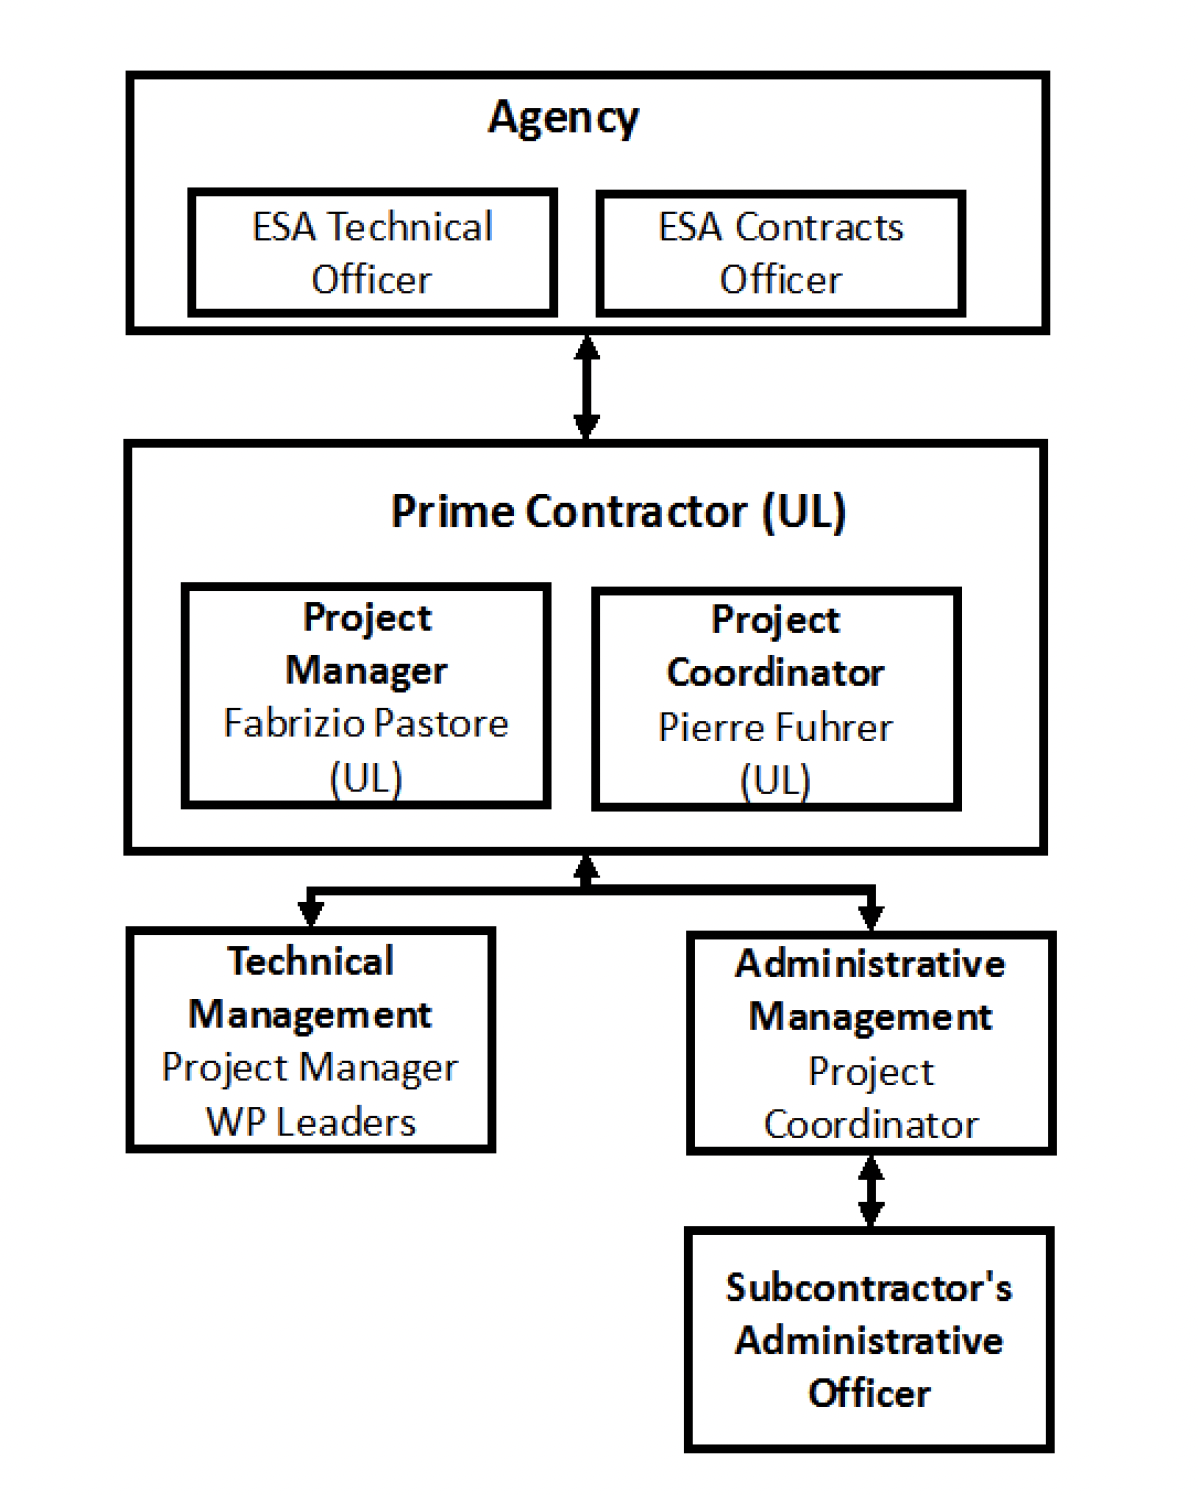
\includegraphics[width=0.5\textwidth]{images/reporting_lines}
\end{figure}

\subsection{Management Objectives and Priorities}

The toolset will be developed by Snt following the defined milestones and validated in tandem with the project partners, with a focus on the following tasks:
\begin{enumerate}
  \item Analysis and survey of mutation testing
  \item Study of mutation testing applicability to space software
  \item Development of the mutation testing framework
  \item Evaluation of mutation testing process and methodology
definition
  \item Maintenance and improvement of the toolset.
\end{enumerate}

\subsection{Master Schedule}

Figure~\ref{fig:GANTT} shows the GANTT chart for the FAQAS project.
The keyword WPx.y and WPx.y.z is used to indicate a task that may have subtasks. The keywords TRx and TMx are used to indicate reviews and task milestones based on SoW. Reviews and milestones are depicted using red and green diamonds, respectively. The critical path is depicted in red and derives from the dependencies between the reviews and the beginning of the following tasks.

\begin{figure}[h]
\caption{GANTT chart for the activity.}
\label{fig:GANTT}
\centering
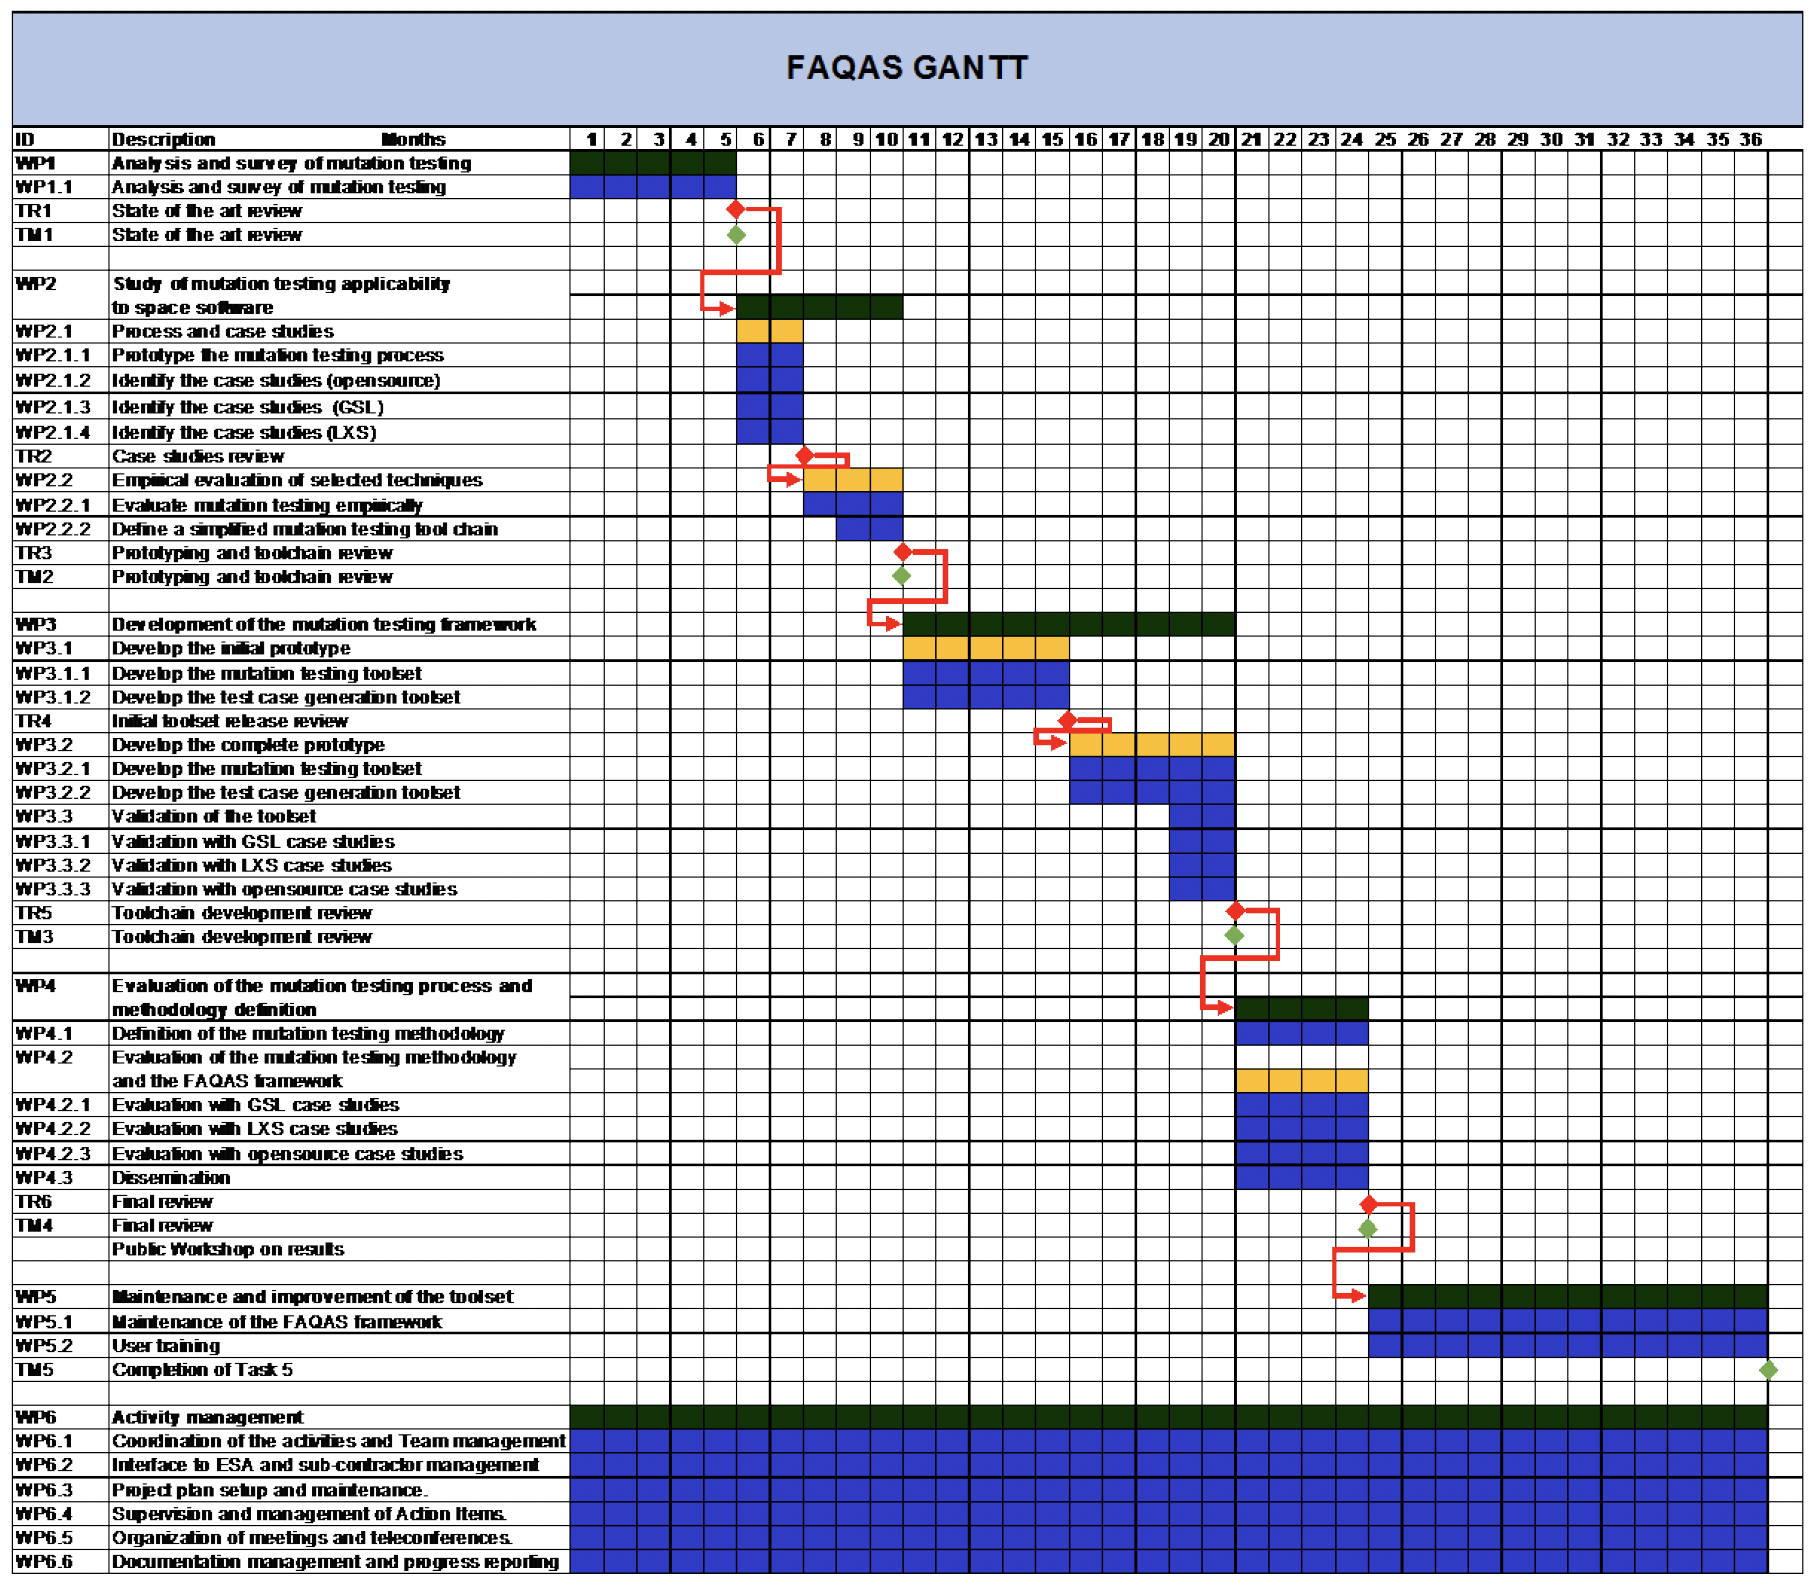
\includegraphics[width=\textwidth]{images/gantt}
\end{figure}

\subsection{Work Breakdown Structure}

Figure~\ref{fig:work_breakdown} shows the work breakdown structure. White boxes show work packages. Gray boxes show tasks within work packages. Boxes with thick lines correspond to tasks and work packages at the end of which a control milestone has been set. Work package and task identifiers match the ones used for the GANTT chart presented in the previous paragraph.

\begin{figure}[H]
\caption{Work breakdown structure.}
\label{fig:work_breakdown}
\centering
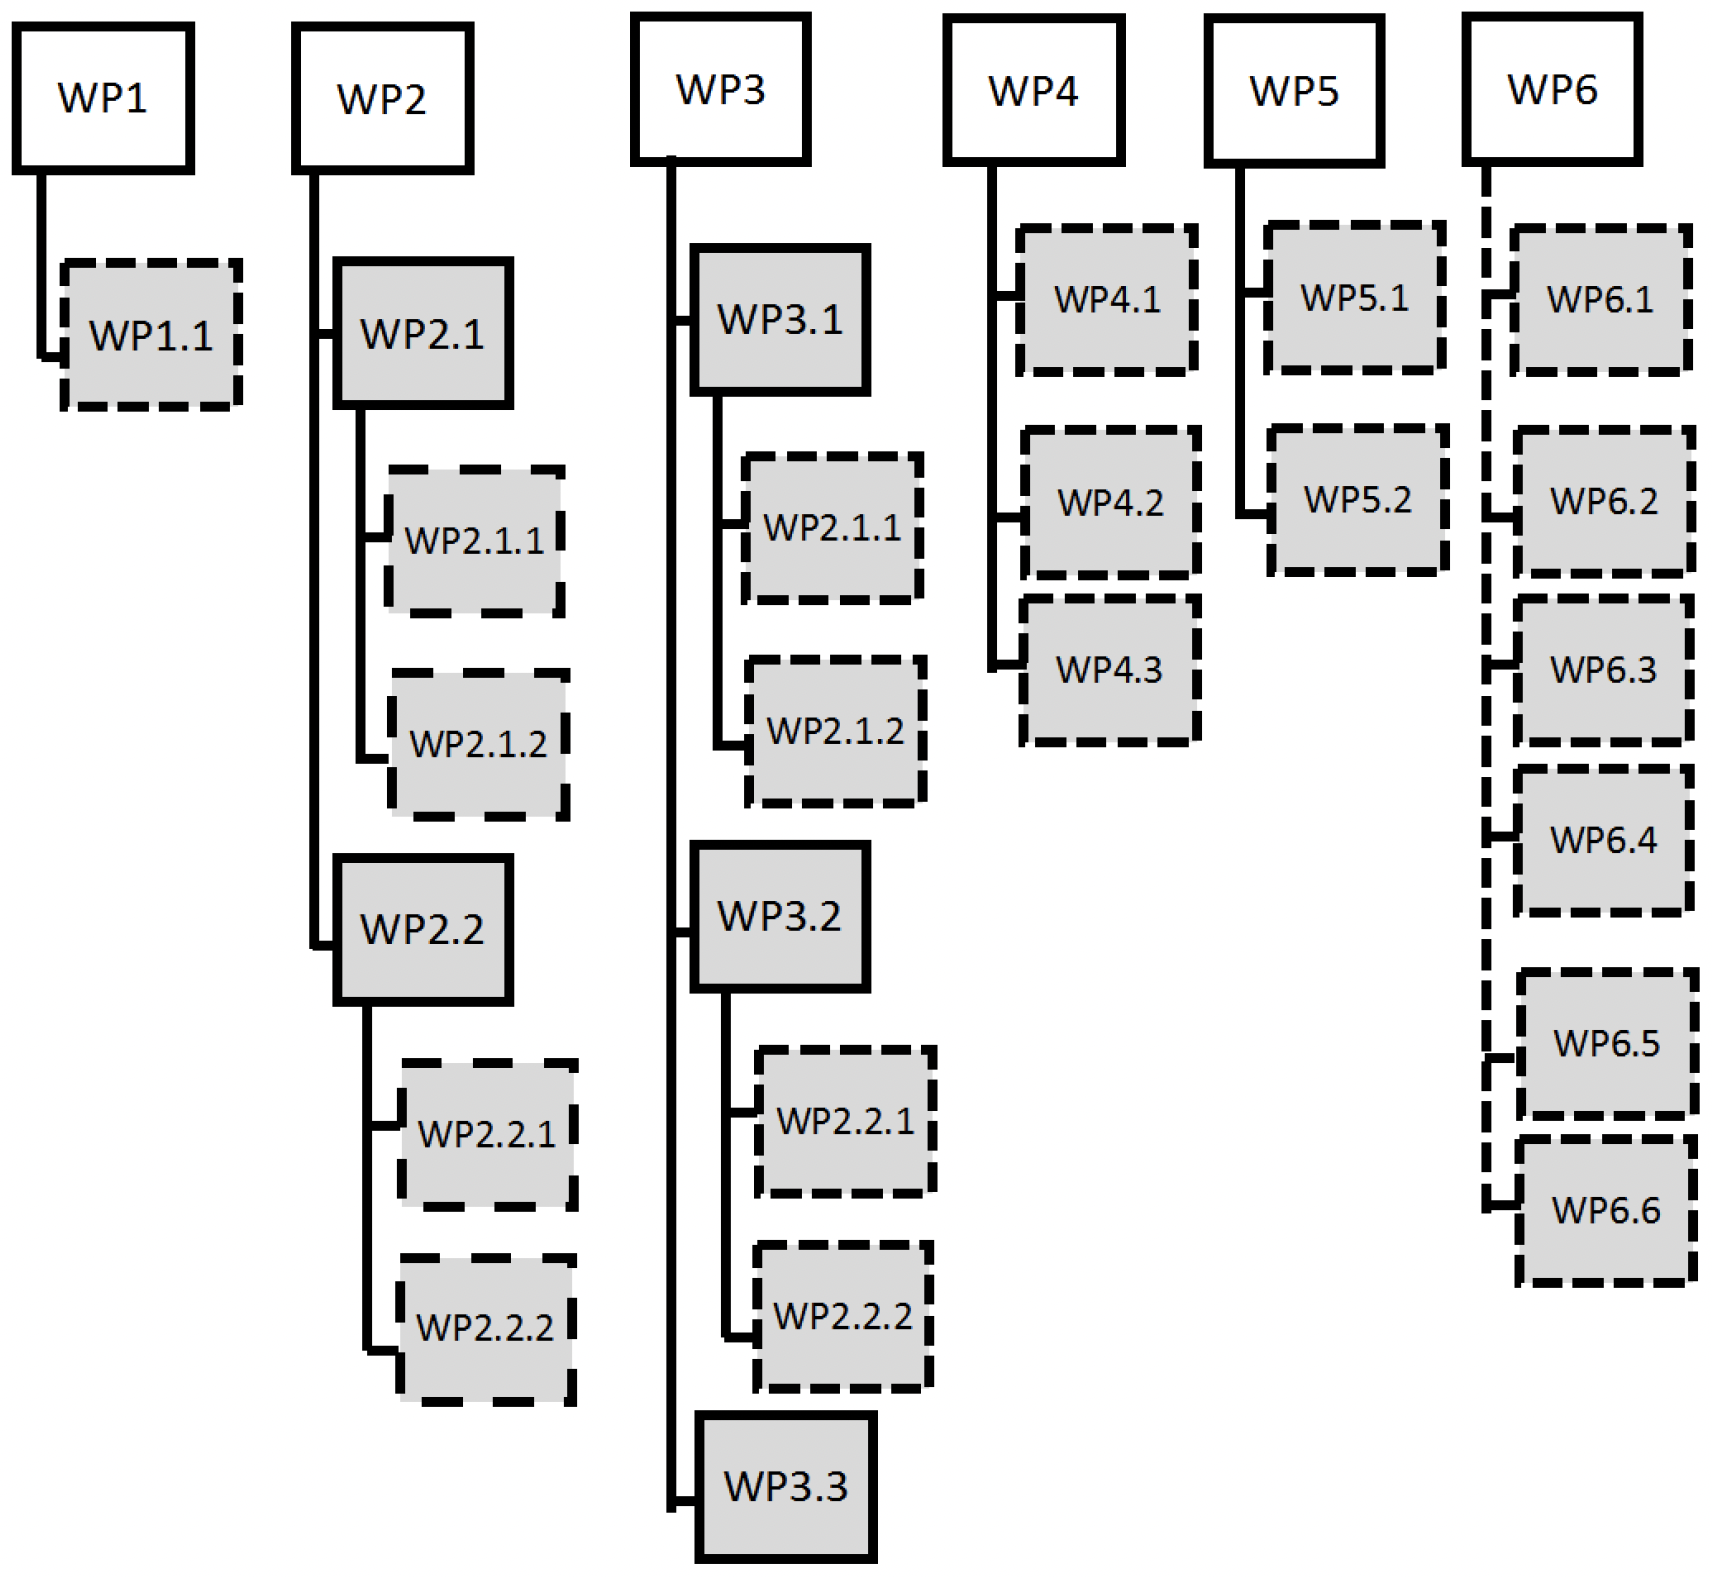
\includegraphics[width=0.5\textwidth]{images/work_breakdown}
\end{figure}

The description of the WP is presented in the following in tabular form.
Every WP is characterized by a list of activities with inputs and outputs consisting of both software and documentation items.

%chiedi a Fabrizio se ha ancora il LateX della technical proposal cosi copio da lí.


\subsection{Monitoring and Controlling Mechanism}

The following monitoring and controlling mechanisms are in place:
\begin{itemize}
  \item Progress meetings
  \item Progress reports
  \item Reviews by partners.
\end{itemize}

\section{Software Development Approach}

The FAQAS framework is composed by the following software tools:
\begin{itemize}
  \item \MASS
  \item \DAMA
  \item \SEMUS
\end{itemize}

Every tool will be developed in accordance with the SSS and RB and validated through the use of unit testing and application to the selected case studies.
The project partners will also evaluate the toolset.


\clearpage
% !TEX root = MAIN.tex

\chapter{Software product quality assurance}

% a.	The SPAP shall describe the approach taken to ensure the quality of the software product.
% b.	The description of the approach specified in B.2.1<7>a shall include the:
% 1.	specification of the product metrics, their target values and the means to collect them;
% 2.	definition of a timely metrication programme;
% 3.	analyses to be performed on the collected metrics;
% 4.	way the results are fed back to the development team;
% 5.	documentation quality requirements;
% 6.	assurance activities meant to ensure that the product meets the quality requirements.
%

\section{Approach}

In this project, the verification and validation of the different software that compose the \FAQAS (i.e., \MASS, \SEMUS, and \DAMA) is performed at two levels: (1) unit test level, and (2) system test level.

\subsection{Unit Testing}

At this level, we assess the quality of single, encapsulated components. In other words, components that do not interact with other units, but simply store results in files processed by other units.

Given its characteristics, we followed this procedure to assess the component \texttt{SRCMutation} from \MASS, and the component \texttt{DDMutation} from \DAMA.

\subsubsection{MASS: SRCMutation}

\begin{figure}[t]
  \centering
  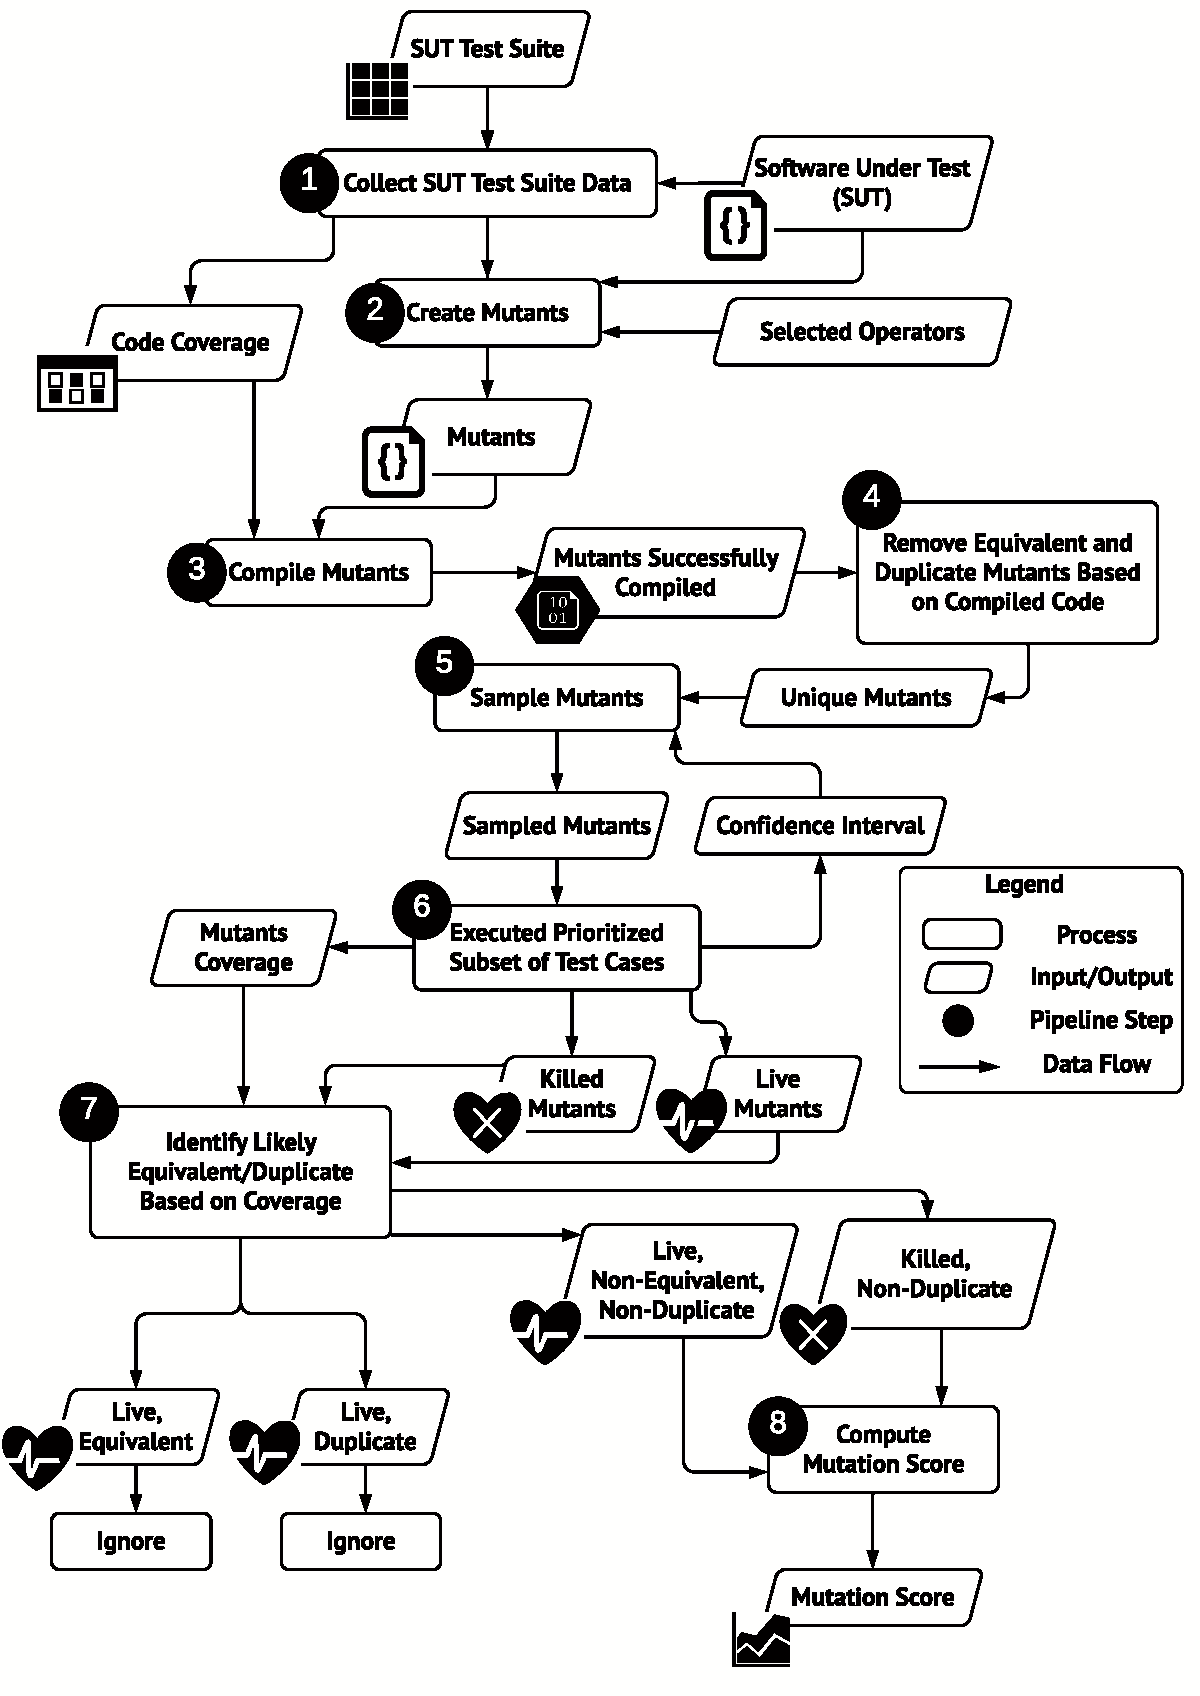
\includegraphics[width=0.6\textwidth]{images/Approach.pdf}
      \caption{MASS methodology.}
      \label{fig:mass}
\end{figure}

Figure~\ref{fig:mass} introduces \MASS methodology. The component \texttt{SRCMutation} is implemented in step 2 of the methodology under the name of \emph{Create Mutants}.

\texttt{SRCMutation} is the component with the most complicate implementation logic and thus it requires a detailed unit testing. All the other components either filter or join data, so their implementation is simpler and thus their test automation is performed through system tests.

For more details, please refer to Chapter 7 of the SUITP document.


\subsubsection{DAMAt: DDMutation}
\TODO{ENRICO, please complete}

\begin{figure}[t]
  \centering
  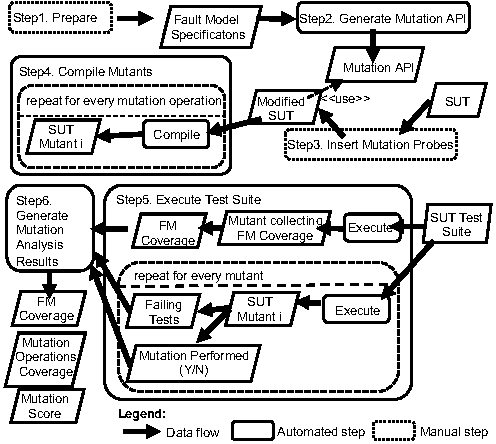
\includegraphics[width=0.6\textwidth]{images/dataDrivenBufferProcess.pdf}
      \caption{DAMAt methodology.}
      \label{fig:damat}
\end{figure}

Figure~\ref{fig:damat} introduces \MASS methodology. The component \texttt{DDMutation} is implemented in step 2 of the methodology under the name of \emph{Generate Mutation API}.

\texttt{DDMutation} is the component with the most complicate implementation logic and thus it requires a detailed unit testing. All the other components either filter or join data, so their implementation is simpler and thus their test automation is performed through system tests.

For more details, please refer to Chapter 11 of the SUITP document.

\subsection{System Testing}

At this level, we test the system as a whole. In particular, we verify and validate all the functional requirements specified in the Software System Specifications document (SSS), for the three software systems of the \FAQAS.

\subsubsection{MASS}

At a system level, we validate that \MASS is able to process the SUT, SUT test suite, and perform correctly the following steps (1) collect SUT test suite data (e.g., code coverage information), (2) create mutants, (3) compile mutants, (4) disregard equivalent and duplicate mutants based on compiler optimizations, (5) sample mutants, (6) execute a prioritized subset of test case, (7) identify likely equivalent based on code coverage, and (8) compute the mutation score.

We validated the eight steps of \MASS on the MLFS case study, and verified that outputs complied with the system specifications. A full description of the validation of \MASS can be found on the SUM document on Chapter 11.

\subsubsection{SEMuS}

\begin{figure}[t]
  \centering
  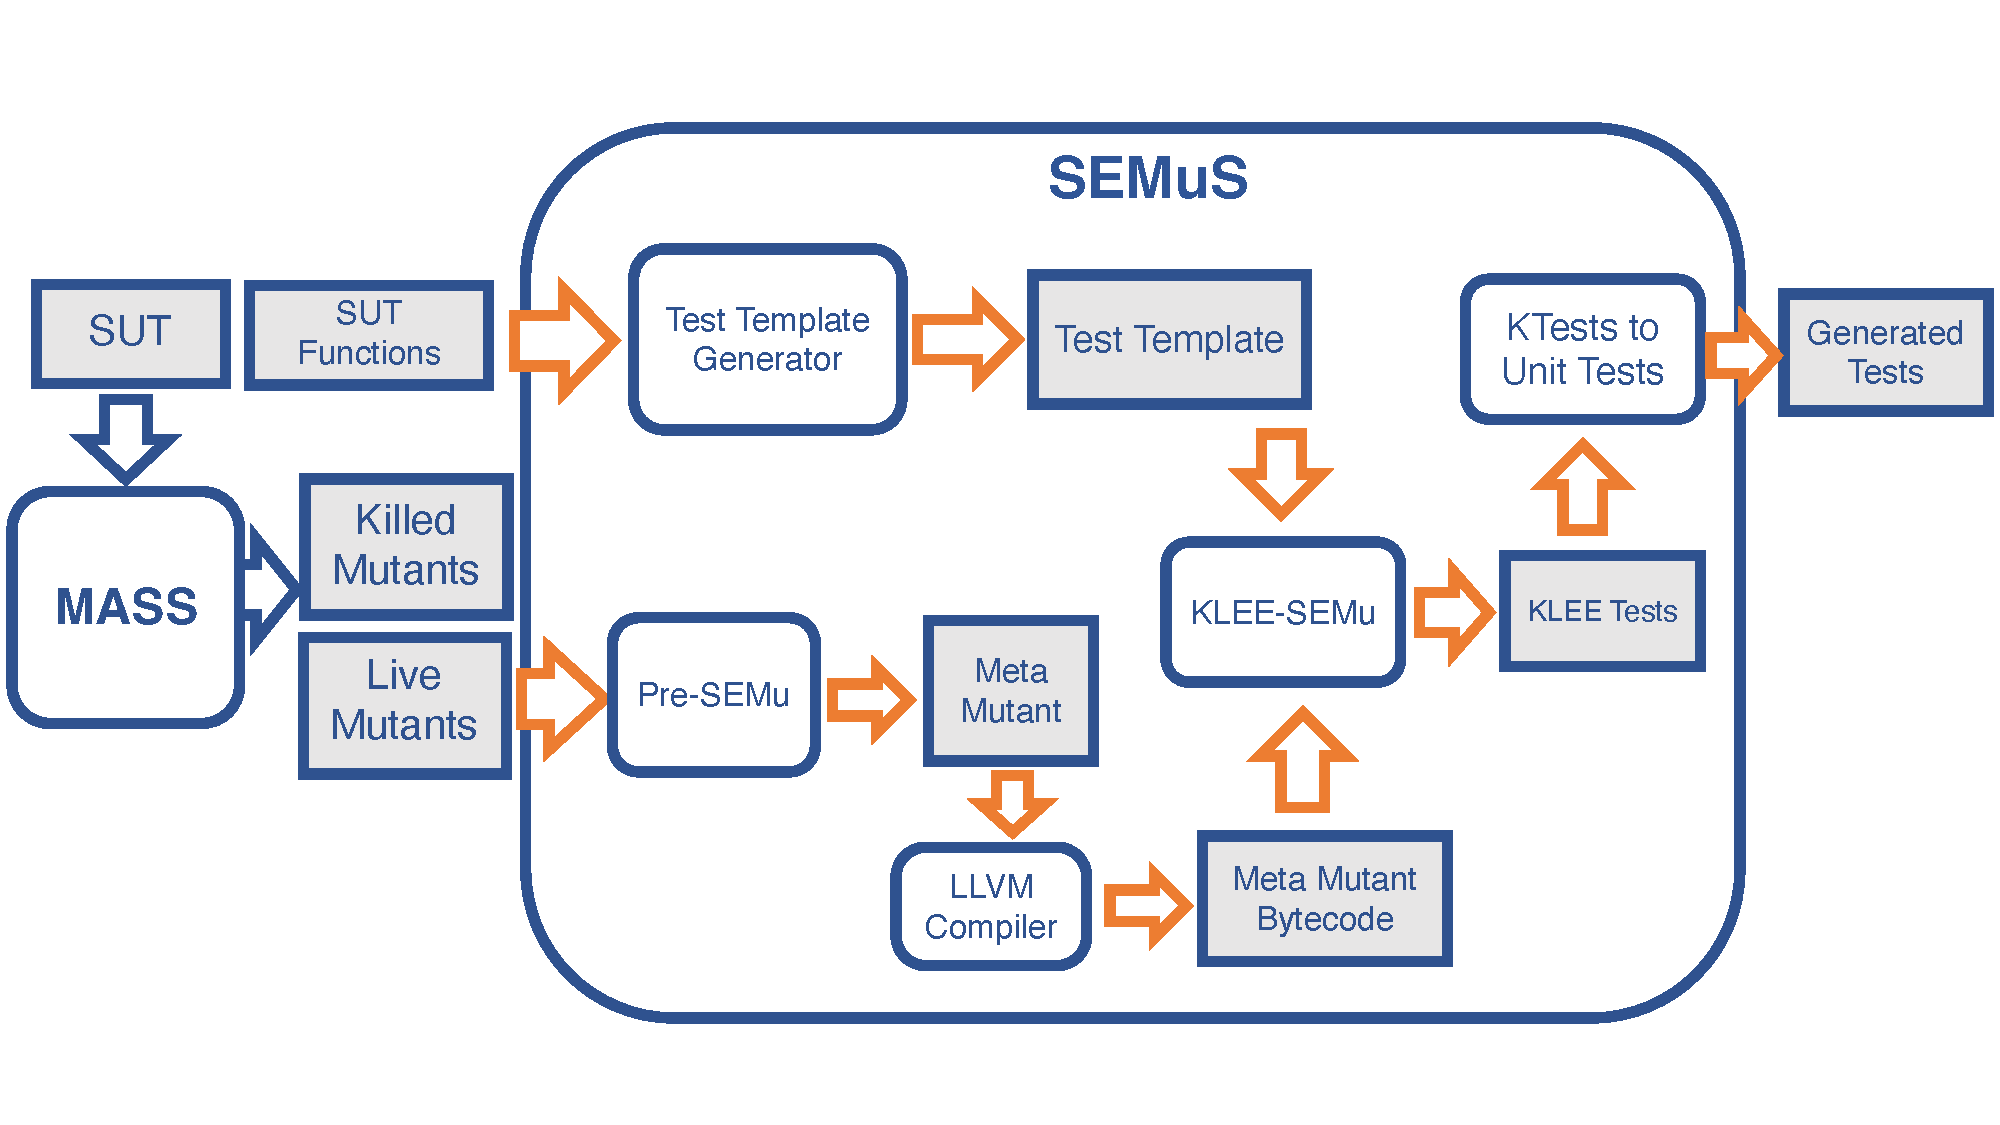
\includegraphics[width=0.8\textwidth]{images/semus-architecture.pdf}
      \caption{SEMuS architecture.}
      \label{fig:semus}
\end{figure}

Figure~\ref{fig:semus} introduces the \SEMUS architecture, and in particular the different inputs and outputs to be considered for verification and validation.

At a system level, we performed a validation of \SEMUS to assure that every functional requirement is compliant with the Software System Specifications document (SSS) document. Particularly, we verified that \SEMUS was able to parse the SUT source code, and perform correctly the following steps (as shown in Figure~\ref{fig:semus}) (1) generate test templates from SUT functions, (2) generate the meta-mutants containing all the live mutants of SUT test suite, (3) compile the meta-mutant and to invoke KLEE-SEMu to trigger the test generation step, and (4) to process the KLEE tests and to convert them to C readable unit test cases.

We validated the four steps of the methodology on the MLFS case study, we also verified that outputs are in line with system specifications. A detailed description of the validation of \SEMUS can be found on the SUM document on Chapter 12.


\subsubsection{DAMAt}

At a system level, we performed a validation of \DAMA to assure that every functional requirement is compliant with the Software System Specifications document (SSS) document.
Particularly, we verified that \DAMA was able to:
\begin{enumerate}
	\item Parse a fault model prepared by the user.
	\item Generate a mutation API with the functions that modify the data according to the provided fault model.
  \item Modify the buffer through calls to the mutation API.
	\item Generate and compile mutants.
	\item Execute the test suite against all the mutants and gather the results of the test cases.
	\item Generate the results of the mutation analysis.
\end{enumerate}

We validated the six steps of the methodology on the following case studies:
\begin{itemize}
  \item LXS System Test Suite for ESAIL
  \item GSL Integration Test Suite for libgscsp
  \item GSL System Test Suite for libparam
\end{itemize}

We also verified that outputs are in line with system specifications. A detailed description of the validation of \DAMA can be found on the D4 document.

\clearpage


\clearpage
% !TEX root = MAIN.tex

\chapter{Software Validation Process Planning}

The validation of the \FAQAS consist of applying it to different case studies provided by LuxSpace and GOMSpace.
Table~\ref{tab:caseStudies} provides the list of case studies and the FAQAS toolset applied on the case studies for validation. Validation is performed after the finalization of each toolset; before its final release. More information about the case studies is reported in \emph{D4}.

\begin{table}[htp]
\caption{Case studies for the FAQAS activity.}
\label{tab:caseStudies}
\begin{center}
\begin{tabular}{|p{1.2cm}|p{6cm}|p{1.5cm}|p{1.5cm}|p{1.5cm}|}
\hline
\textbf{Partner}&\textbf{Case study}&\textbf{MASS}&\textbf{SEMuS}&\textbf{DAMAt}\\
\hline
LXS&System Test Suite for ESAIL&Y&N&Y\\
LXS&Unit Test Suite for ESAIL&Y&N&N\\
GSL&Unit Test Suite for libUtil&Y&Y*&N\\
GSL&Integration Test Suite for libgscsp&Y&N&Y*\\
GSL&System Test Suite for libparam&Y&N&Y\\
ESA&MLFS mathematical library&Y&Y&N\\
ESA&ASN1 Compiler&Y&Y&N\\
\hline
\end{tabular}
\end{center}
An asterisk (*) is used to indicate validation cases that will be finalized in WP4.
\end{table}

\clearpage


\clearpage
% !TEX root = MAIN.tex
\chapter{Software Verification Plan}
The purpose of this Software Verification Plan is to describe the approach and the organization of the software verification activitiess for the components of the FAQAS framework.

It addresses the follwing items:
\begin{itemize}
  \item the software products and life cycle activities
  subject to verification.
  \item the required verification tasks for each life cycle activity, software product, related resources, responsibilities, and schedule.
  \item the procedures for forwarding verification reports to the customer and other involved organizations.
\end{itemize}

\section{Software verification process overview}

\subsection{General}

The FAQAS Framework is comprised by category D classified SW so the verification activities shall be tailored to match this criticality level.

% a. The SVerP shall describe the approach to be utilized to implement the
% verification process throughout the software life cycle, the verification
% effort, and the level of independence for the verification tasks, as follows:
% NOTE 1 It is important to check the applicability of
% ECSS‐Q‐ST‐80 clause 5.3.1 (management of
% risks), 6.2.2 (software dependability and safety)
% and 6.2.6.13 (independent software verification
% and validation).
% NOTE 2 The verification effort is sized according to:
% • the potential for an undetected error in a
% system or software requirement to cause
% death or personal injury, mission failure, or
% financial or catastrophic equipment loss or
% damage;
% • the maturity of and risks associated with the
% software technology to be used;
% • availability of funds and resources.

\subsection{Organization}

% a. The SVerP shall describe the organization of the documentation review,
% proofs, and tracing activities.
% b. The following topics that shall be included:
% 1. roles;
% 2. reporting channels;
% 3. levels of authority for resolving problems;
% 4. organization relationships;
% 5. level of required and implemented independence.

\subsection{Master Schedule}

% a. A reference to the master schedule given in the software development
% plan shall be done.
% b. This SVerP shall describe the schedule for the planned verification
% activities.

\subsection{Resource summary}

% a. The SVerP shall summarize the resources to be used to perform the
% verification activities such as staff, hardware and software tools.

\subsection{Responsibilities}

% a. The SVerP shall describe the specific responsibilities.

\subsection{Identification of risks and level of independence.}

% a. The SVerP shall state (or refer to the SDP) the risks and level of
% independence.

\subsection{Tools, techniques and methods}

% a. The SVerP shall describe the software tools, techniques and methods
% used to execute the verification tasks throughout the software life cycle.

\subsection{Control procedures for verification process}

% a. The SVerP shall contain information (or reference to) about applicable
% management procedures concerning the following aspects:
% 1. problem reporting and resolution;
% 2. deviation and waiver policy;

\section{Verification activities}

\subsection{General}

% a. The SVerP shall address the verification activities of each software item.
% b. The SVerP shall address separately the activities to be performed for
% manually and automatically generated code.

\subsection{Software process verification}

% a. For each software process verification, the SVerP shall list:
% 1. the verification activities to be performed and how they are
% performed.
% 2. the required inputs to achieve the verification activities.
% 3. the intermediate and final outputs documenting the performed
% verification activities.
% 4. the methodologies, tools and facilities utilized to accomplish the
% verification activities.
% NOTE Examples of input and output are:
% • for software requirements (RB and TS) and
% architecture engineering:
% • input: draft SRS, draft software architectural
% design
% • output: software verification requirements
% report, software architectural design to
% requirements traceability
% • for software design and implementation
% engineering:
% • input: software components design, code,
% software user manual, software integration
% test plan
% • output: software code verification report,
% evaluation of software validation testing
% specification
% • for software delivery and acceptance:
% • input: software validation specification with
% respect to the requirements baseline,
% software acceptance testing documentation
% • output: software acceptance test report,
% software acceptance data package, problem
% reports, software release document,
% software configuration file
% • for software validation:
% • input: software validation specification with
% respect to the requirements baseline
% • output: software validation testing
% specifications

\subsection{Software quality requirements verification (as per ECSS‐QST‐80 clause 6.2.6.1)}

% <6.3.1> Activities
% a. The SVerP shall list the verification activities to be performed and how
% these are accomplished.
% NOTE Verification includes various techniques such as
% review, inspection, testing, walk‐through,
% cross‐reading, desk‐checking, model
% simulation, and many types of analysis such astraceability analysis, formal proof or fault tree
% analysis.
% <6.3.2> Inputs
% a. The SVerP shall list the required inputs to accomplish the verification
% activities.
% <6.3.3> Outputs
% a. The SVerP shall list the intermediate and final outputs documenting the
% performed verification activities.
% <6.3.4> Methodology, tools and facilities
% a. The SVerP shall describe the methodologies, tools and facilities utilized
% to accomplish the software quality requirements verification activities.


\clearpage
% !TEX root = MAIN.tex
\chapter{Software Maintenance Plan}
\label{chapter:maintenance}
% This document is the Software Maintenance Plan (SMP) for the Basic mathematical Library (BL) and the Basic mathematical Library Test Suite (BLTS) of the Mathematical Library for Flight Software (MLFS) project. It is composed of this document itself, its accompanying resources for the maintenance tasks E1356-GTD-SMP-01a, and the template for NCR submission E1356-GTD-SMP-01b.
% Its purpose is to provide the definition of organizational aspects and management approach to the implementation of the maintenance tasks and to describe the approach to the implementation of the maintenance process for this software product.
% GTD GmbH developed the software but the maintenance of the MLFS library is not part of the contract, thus this plan will define how to act in case of a required maintenance but will not define resources and schedule aspects of the maintenance process.
% The software maintenance plan is a constituent of the maintenance file (MF).

% 6.3.8.1
% a. The organization responsible for maintenance shall be identified to allow a smooth transition into the operations and maintenance.
% NOTE An organization, with representatives from both supplier and customer, can be set up to support the maintenance activities. Attention is drawn to the importance of the flexibility of this organization to cope with the unexpected occurrence of problems and the identification of facilities and resources to be used for the maintenance activities.
% EXPECTED OUTPUT: Maintenance plan [MF, -; QR, AR, ORR].
% 6.3.8.2
% a. The maintenance organization shall specify the assurance, verification and validation activities applicable to maintenance interventions.
% EXPECTED OUTPUT: Maintenance plan [MF, -; QR, AR, ORR].
% 6.3.8.3
% a. The maintenance plans shall be verified against specified requirements for maintenance of the software product.
% NOTE The maintenance plans and procedures can address corrective, improving, adaptive and preventive maintenance, differentiating between “routine” and “emergency” maintenance activities.
% 6.3.8.4
% a. The maintenance plans and procedures shall include the following as a minimum:
% 1. scope of maintenance;
% 2. identification of the first version of the software product for which maintenance is to be done;
% 3. support organization;
% 4. maintenance life cycle;
% 5. maintenance activities;
% 6. quality measures to be applied during the maintenance;
% 7. maintenance records and reports.
% EXPECTED OUTPUT: Maintenance plan [MF, -; QR, AR, ORR].

% To support the adoption of the FAQAS framework, SnT will guarantee a maintenance period of 12 months after the end of the activity. The FAQAS framework will be made available through code hosting services (e.g., GitHub[36] and GitLab[37]), likely the Gitlab service of the University of Luxembourg [38]. Built-in issue tracking features will be used to track bug requests and fixes.
% SnT will guarantee corrective, adaptive and preventive maintenance [R5-2] except for exceptional case that imply a major rewriting of the toolset. Such cases will be likely included in the methodology definition as corner cases where the current toolsets cannot be applied.
% Activities related to training [R5-3], documentation [R5-4], and software releases [R5-5] will be performed according to SoW.

This Chapter contains the Software Maintenance Plan (SMP) for the FAQAS framework.

\section{Scope and Purpose}

Its purpose is to provide the definition of organizational aspects and management approach to the implementation of the maintenance tasks and to describe the approach to the implementation of the maintenance process for this software product.

\section{Application of the Plan}

 The FAQAS framework will be made available through code hosting services (i.e., the Gitlab service of ESA\footnote{https://gitrepos.estec.esa.int/external/FAQAS}). Built-in issue tracking features will be used to track bug requests and fixes.

\section{Maintenance Concept}

To support the adoption of the FAQAS framework, SnT will guarantee a maintenance period of 12 months after the end of the activity.
SnT will guarantee corrective, adaptive and preventive maintenance except for exceptional case that imply a major rewriting of the toolset.
Such cases will be included in the methodology definition as corner cases where the current toolsets cannot be applied.


% \clearpage
% % !TEX root = MAIN.tex
\chapter{Software Product Assurance Plan}

% The supplier shall develop a software product assurance plan in response to the software product assurance requirements in conformance with DRD in annex B.
% b. The software product assurance plan shall be either a standalone document or a section of the supplier overall product assurance plan.

% a. Testing shall be performed in accordance with a strategy for each testing level (i.e. unit, integration, validation against the technical specification, validation against the requirements baseline, acceptance), which includes:
% 1. the types of tests to be performed;
% NOTE For example: functional, boundary, performance, and usability tests.
% 2. the tests to be performed in accordance with the plans and procedures;
% 3. the means and organizations to perform assurance function for testing and validation.
% EXPECTED OUTPUT: Software product assurance plan [PAF, SPAP; PDR, CDR].

% 6.3.5.2
% a. Based on the criticality of the software, test coverage goals for each testing level shall be agreed between the customer and the supplier and their achievement monitored by metrics:
% 1. for unit level testing;
% 2. for integration level testing;
% 3. for validation against the technical specification and validation against the requirements baseline.
% EXPECTED OUTPUT: Software product assurance plan [PAF, SPAP; PDR, CDR].
% 6.3.5.3
% a. The supplier shall ensure through internal review that the test procedures and data are adequate, feasible and traceable and that they satisfy the requirements.
% EXPECTED OUTPUT: Software product assurance reports [PAF, -; -].
% 6.3.5.4
% a. Test readiness reviews shall be held before the commencement of test activities, as defined in the software development plan.
% EXPECTED OUTPUT: Test readiness review reports [DJF, -; TRR].

% 6.3.5.5
% a. Test coverage shall be checked with respect to the stated goals.
% EXPECTED OUTPUT: Software product assurance reports [PAF, -; -].
% b. Feedback from the results of test coverage evaluation shall be continuously provided to the software developers.
% 6.3.5.6
% a. The supplier shall ensure that nonconformances and software problem reports detected during testing are properly documented and reported to those concerned.
% EXPECTED OUTPUT: Nonconformance reports and software problem reports [DJF, -; CDR, QR, AR, ORR].
% 6.3.5.7
% a. The test coverage of configurable code shall be checked to ensure that the stated requirements are met in each tested configuration.
% EXPECTED OUTPUT: Statement of compliance with test plans and procedures [PAF, -; CDR, QR, AR, ORR].
% 6.3.5.8
% a. The completion of actions related to software problem reports generated during testing and validation shall be verified and recorded.
% EXPECTED OUTPUT: Software problem reports [DJF,

% 6.3.5.12
% a. The supplier shall ensure that tests are repeatable by verifying the storage and recording of tested software, support software, test environment, supporting documents and problems found.
% EXPECTED OUTPUT: Software product assurance reports [PAF, -; -].
% 6.3.5.13
% a. The supplier shall confirm in writing that the tests are successfully completed.
% EXPECTED OUTPUT: Testing and validation reports [DJF, -; CDR, QR, AR, ORR].
%
% 6.3.5.11
% a. The supplier shall ensure that:
% 1. tests are conducted in accordance with approved test procedures and data,
% 2. the configuration under test is correct,
% 3. the tests are properly documented, and
% 4. the test reports are up to date and valid.
% EXPECTED OUTPUT: Statement of compliance with test plans and procedures [PAF, -; CDR, QR, AR, ORR].

% 6.3.5.15
% a. Areas affected by any modification shall be identified and re‐tested (regression testing).
% 6.3.5.16
% a. In case of re‐testing, all test related documentation (test procedures, data and reports) shall be updated accordingly.
% EXPECTED OUTPUT: Updated test documentation [DJF, -; CDR, QR, AR, ORR].

% 6.3.5.18
% a. The need for regression testing and additional verification of the software shall be analysed after a change or update of any tool used to generate it.
% NOTE For example: source code or object code.
% EXPECTED OUTPUT: Updated test documentation

% 7.1.3 Assurance activities for product quality requirements
% a. The supplier shall define assurance activities to ensure that the product meets the quality requirements as specified in the technical specification.
% EXPECTED OUTPUT: Software product assurance plan [PAF, SPAP; SRR, PDR].

\section{Software product assurance programme implementation}

\subsection{Organization}
\label{subsec:organization}
% a. The SPAP shall describe the organization of software product assurance activities, including responsibility, authority and the interrelation of personnel who manage, perform and verify work affecting software quality.
% b. The following topics shall be included:
% 1. organizational structure;
% 2. interfaces of each organisation, either external or internal, involved in the project;
% 3. relationship to the system level product assurance and safety;
% 4. independence of the software product assurance function;
% 5. delegation of software product assurance tasks to a lower level supplier, if any

The product assurance activities will be performed following the team organization defined in Chapter~\ref{chapter:organization}.

\subsection{Reporting}
% The reporting related to product assurance processes includes:
SnT shall report on a regular basis on the status of the software product assurance programme implementation, as part of the overall reporting of the project.

\subsection{Quality models}
% a. The SPAP shall describe the quality models applicable to the project and how they are used to specify the quality requirements.
% Quality models shall be used to specify the software quality requirements.

\subsection{Methods and tools}
% a. The SPAP shall describe the methods and tools used for all the activities of the development cycle, and their level of maturity.

The methods and tools used for the activities of the development cycle are described in Chapter~\ref{chapter:software_development} and in Chapter~\ref{chapter:organization}.

The PA Manager will ensure that:
\begin{itemize}
  \item the development team has adequate experience and training to make use of  the methods and tools.
  \item the tools and methods are appropriate for the characteristics of the product in development.
  \item the tools and relative hardware are available throughout the lifetime of the product.
  \item the methods and tools are correctly used.
\end{itemize}


\subsection{Operation and Maintenance}
For the maintenance phase a software maintenance plan shall be prepared.
The outline shall be described in Chapter~\ref{chapter:maintenance}.

\subsection{Software problems}

Software problems will be managed throught GitLab built-in issue tracking features as described in Chapter~\ref{chapter:maintenance}.



% % !TEX root = MAIN.tex

\chapter{Compliance matrix to software product assurance requirements}

% a.	The SPAP shall include the compliance matrix to the applicable software product assurance requirements (e.g. ECSS-Q-ST-80 clauses, as tailored by a product assurance requirements document), or provide a reference to it.
% b.	For each software product assurance requirement, the following information shall be provided:
% 1.	requirement identifier;
% 2.	compliance
% (C = compliant, NC = non–compliant, NA = not applicable);
% 3.	reference to the project documentation covering the requirement (e.g. section of the software product assurance plan);
% 4.	remarks.



\clearpage



% \newpage
% % !TEX root = MAIN.tex
\chapter{ESA Revisions}

%% !TEX root = MAIN.tex

\section{Responses to ESA comments provided on 12.04.2021}
\label{sec:ESA:comments:1}

Comments IDs appear also in the main document next to the text modified to address the comment. To save space in the main text, the prefix \emph{ITSR-SSS-PABG-} has been abbreviated as \emph{P-}.

\setlength\LTleft{0pt}
\setlength\LTright{0pt}
\tiny 
%@{\extracolsep{\fill}}
\begin{longtable}{|p{1.5cm}|p{12cm}|@{}}
%\caption{\normalsize .}
%\label{table:comments:responses} 
\textbf{Comment ID}&\textbf{Response}\\
\\
\hline
P-1&
\begin{minipage}{12cm}
We will need to discuss the detail of the merge of the two specifications during the review meeting.
\end{minipage}\\
\\
\hline

P-2&
\begin{minipage}{12cm}
Done.
\end{minipage}\\
\\
\hline

P-3&
\begin{minipage}{12cm}
Done.
\end{minipage}\\
\\
\hline

P-4&
\begin{minipage}{12cm}
Done.
\end{minipage}\\
\\
\hline

P-5&
\begin{minipage}{12cm}
Done.
\end{minipage}\\
\\
\hline

P-6&
\begin{minipage}{12cm}
Done.
\end{minipage}\\
\\
\hline

P-7&
\begin{minipage}{12cm}
Done.
\end{minipage}\\
\\
\hline

P-8&
\begin{minipage}{12cm}
Done.
\end{minipage}\\
\\
\hline

P-9&
\begin{minipage}{12cm}
It is worth discussing if it makes sense to perform mutation analysis without code coverage.
\end{minipage}\\
\\
\hline


P-10&
\begin{minipage}{12cm}
We always generate all the mutants because it's fast. End-users have the option to execute a subset of them.
\end{minipage}\\
\\
\hline

P-11&
\begin{minipage}{12cm}
We changed a sentence, but this requirement is long because we had to provide an explanation missing from D2.
\end{minipage}\\
\\
\hline

P-12&
\begin{minipage}{12cm}
\end{minipage}\\
\\
\hline

P-13&
\begin{minipage}{12cm}
\end{minipage}\\
See P-8\\
\hline

P-14&
\begin{minipage}{12cm}
\end{minipage}\\
Action item. To be done for the end of WP3.\\
\hline


P-15&
\begin{minipage}{12cm}
TOD
\end{minipage}\\
\hline

P-16&
\begin{minipage}{12cm}
Done.
\end{minipage}\\
\hline

P-17&
\begin{minipage}{12cm}
We will provide a table for end of WP3.
\end{minipage}\\
\hline
                                                
\end{longtable}
\normalsize

\clearpage

% !TEX root = MutationTestingSurvey.tex

\section{Responses to ESA comments provided on 03.04.2020}
\label{sec:ESA:comments:2}


\setlength\LTleft{0pt}
\setlength\LTright{0pt}
\tiny 
\begin{longtable}{|p{1.5cm}|p{12cm}|@{}}
\label{table:comments:responses} 
\textbf{Comment ID}&\textbf{Comment and Response (below)}\\
\\
\midrule
C6 \& C7
&
Have you seen numbers for this mutation score and threshold in the literature? Is this something to be checked during the use case evaluation?
\\
\cmidrule{2-2}
&
We have addressed the comments above.
\TODO{OScar: please check if the survey of Papadakis say something aboth teh threshold (C7)}
\\
\hline
C8
&
Elaborate a bit more on C8 (pros and cons of doing mutation at source code / IR/ Assembly/ Executable);
\\
\cmidrule{2-2}
&
\TODO{Oscar: you may refer to taht paper of Darko Marinov and Co. to say IR is not good}
\\
\hline
C31
&
What is this sufficient set of operators?
\\
\cmidrule{2-2}
&
\TODO{Oscar}
\\
\hline
C32
&
Can you please add the solution for this example? i.e. do we need two different test cases of isPalindrome to detect both mutants?
\\
\cmidrule{2-2}
&
\TODO{Oscar}
\\
\hline
C33
&
Even if the objectives are complementary, both of them should be pursued for a data mutation testing approach?
\\
\cmidrule{2-2}
&
We have addressed the comment above.
\\
\hline
C34
&
The sentence sounds weird... To automate?? Is this activity something that can be automated?
\\
\cmidrule{2-2}
&
We have addressed the comment above by clarifying our text.
\\
\hline
C35
&
Is it possible to add an example of equivalent and redundant mutants?
\\
\cmidrule{2-2}
&
We have added the requested examples.
\\
\hline
C36
&
\begin{minipage}{12cm}
Related to automation, in my opinion, what it is key is that the test assessment process (for both data and code mutation) is as much automated as possible.\\

Automated generation of test cases is a very nice to have. In an industrial environment, let's say that we could afford spending some time to manually augment the test suite.\\

You may consider this to prioritize tasks within this activity.
\end{minipage}
\\
\cmidrule{2-2}
&
We agree on the comment. No need to change the text in this deliverable.
\\
\hline
C37
&
Are we missing a chapter to address the Generation of Test Oracles?\\
\cmidrule{2-2}
&
We have added a section concerning generation of test oracles for code-driven mutation testing (Section~\ref{sec:oraclesGeneration:codeDriven}) and data-driven mutation testing 
(Section~\ref{sec:oracles:dataMutation}).
\\
\hline
C38
&
\begin{minipage}{12cm}
a. From these Case Studies, is there any that you would like to try out within FAQAS?\\

b. One thing that we may need for FAQAS framework is to have kind of a test suite allowing to test the tool, and also to test the tool when new versions will be produced. Would any of these case studies fulfill that?
\end{minipage}
\\
\cmidrule{2-2}
&
We have discussed this topics by voice.
\\
\hline
C39
&
Do you have any information on the kind of test suite? (e.g. is it unit testing, system testing, ...)
\\
\cmidrule{2-2}
&
\TODO{}
\\
\hline
C40
&
Are these case studies focused on Code-Mutation, Data-Mutation, or both?\\
\cmidrule{2-2}
&
\TODO{}
\\
\hline
C41
&
Is there any meaningful conclusion (positive or negative) from those industrial case studies?\\
\cmidrule{2-2}
&
\TODO{}
\\
\hline
C42
&
\begin{minipage}{12cm}
Can we make a conclusion paragraph on this?\\

e.g. No tool based on mutation testing is known to be used within an industrial software development environment\\
e.g. Mutation testing is seen applied mainly within research environments\\
etc, etc
\end{minipage}
\\
\cmidrule{2-2}
&
\TODO{}
\\
\hline
C43
&
Is there any of these trends that could be meaningful to explore?
\\
\cmidrule{2-2}
&
\TODO{}
\\
\hline
C44
&
\begin{minipage}{12cm}
	\begin{itemize}
		\item Is there any particular trend for Code-Based mutation testing? (e.g. research is on-going or vanishing, the way to apply it, the type of operators used, the tools supporting it, ...)
		\item Any particular trend for Data-Based mutation testing?
	\end{itemize}
\end{minipage}
\\
\cmidrule{2-2}
&
\TODO{}
\\
\hline
C45&
\begin{minipage}{12cm}
D1 is fulfilling well requirement R1-1 as in the SoW. There is only one exception, on the red sentence below:\\

[R1-1.c] The applications of mutation testing (e.g. code and data mutation, test-suite evaluation, test cases generation, test-data generation, \textcolor{red}{code quality improvement}, ...)\\

The evaluation of code quality improvement is to be looked at. Indeed, this would be a secondary objective of applying mutation testing on space systems, but we would like to understand if mutation testing could help improve the code quality or not.\\
\end{minipage}
\\
\cmidrule{2-2}
&
\begin{minipage}{12cm}
We added a paragraph on Chapter~\ref{chapter:trends} explaining that there are no works in literature about quality code improvement based on code-driven mutation testing.
\end{minipage}
\\

\bottomrule                                                             
\end{longtable}
\normalsize

\clearpage



\clearpage

\printindex

\end{document}
